\documentclass[11pt]{article}
\usepackage[paperwidth=13.333in,paperheight=7.5in,margin=0.25in]{geometry}
\pagestyle{empty}
\usepackage{tikz}
\usetikzlibrary{arrows.meta,positioning,fit,calc,shapes.geometric,backgrounds}
\usepackage{xcolor}
% The default palette is the white-background evidence-report style. The
% figure builder defines \DARKTHEME for slide-ready variants.
\ifdefined\DARKTHEME
\definecolor{ink}{HTML}{F3F7FA}
\definecolor{muted}{HTML}{B9C7D4}
\definecolor{grid}{HTML}{2B3B4B}
\definecolor{blue}{HTML}{62B8FF}
\definecolor{teal}{HTML}{55D6C2}
\definecolor{orange}{HTML}{FFBD5A}
\definecolor{red}{HTML}{FF7568}
\definecolor{purple}{HTML}{C3A6FF}
\definecolor{paleBlue}{HTML}{14283A}
\definecolor{paleOrange}{HTML}{3A2B14}
\definecolor{dataFill}{HTML}{241C3A}
\definecolor{modelFill}{HTML}{12352F}
\definecolor{specialistFill}{HTML}{3A2B14}
\definecolor{futureFill}{HTML}{1C2630}
\definecolor{pageBg}{HTML}{080D13}
\else
\definecolor{ink}{HTML}{102A43}
\definecolor{muted}{HTML}{52606D}
\definecolor{grid}{HTML}{D9E2EC}
\definecolor{blue}{HTML}{1976A8}
\definecolor{teal}{HTML}{16817A}
\definecolor{orange}{HTML}{D9822B}
\definecolor{red}{HTML}{C05640}
\definecolor{purple}{HTML}{6B5B95}
\definecolor{paleBlue}{HTML}{E8F1F5}
\definecolor{paleOrange}{HTML}{FFF1DF}
\definecolor{dataFill}{HTML}{F5F0FA}
\definecolor{modelFill}{HTML}{EAF6F4}
\definecolor{specialistFill}{HTML}{FFF1DF}
\definecolor{futureFill}{HTML}{F2F4F5}
\definecolor{pageBg}{HTML}{FFFFFF}
\fi
\pagecolor{pageBg}
\tikzset{
  base/.style={font=\sffamily, text=ink},
  title/.style={base, font=\sffamily\bfseries\fontsize{23}{27}\selectfont},
  subtitle/.style={base, font=\sffamily\fontsize{12}{15}\selectfont, text=muted},
  box/.style={base, rounded corners=3pt, draw=blue!65!black, fill=paleBlue, minimum height=0.78cm, minimum width=2.65cm, align=center, inner sep=7pt},
  data/.style={box, draw=purple!75!black, fill=dataFill},
  model/.style={box, draw=teal!75!black, fill=modelFill},
  specialist/.style={box, draw=orange!85!black, fill=specialistFill},
  future/.style={box, draw=muted, fill=futureFill, dashed},
  arrow/.style={-{Latex[length=3mm]}, line width=0.9pt, draw=muted},
  dashedarrow/.style={-{Latex[length=3mm]}, line width=0.8pt, draw=muted, dashed},
  note/.style={base, font=\sffamily\fontsize{18}{22}\selectfont, text=muted, align=left},
}

\begin{document}
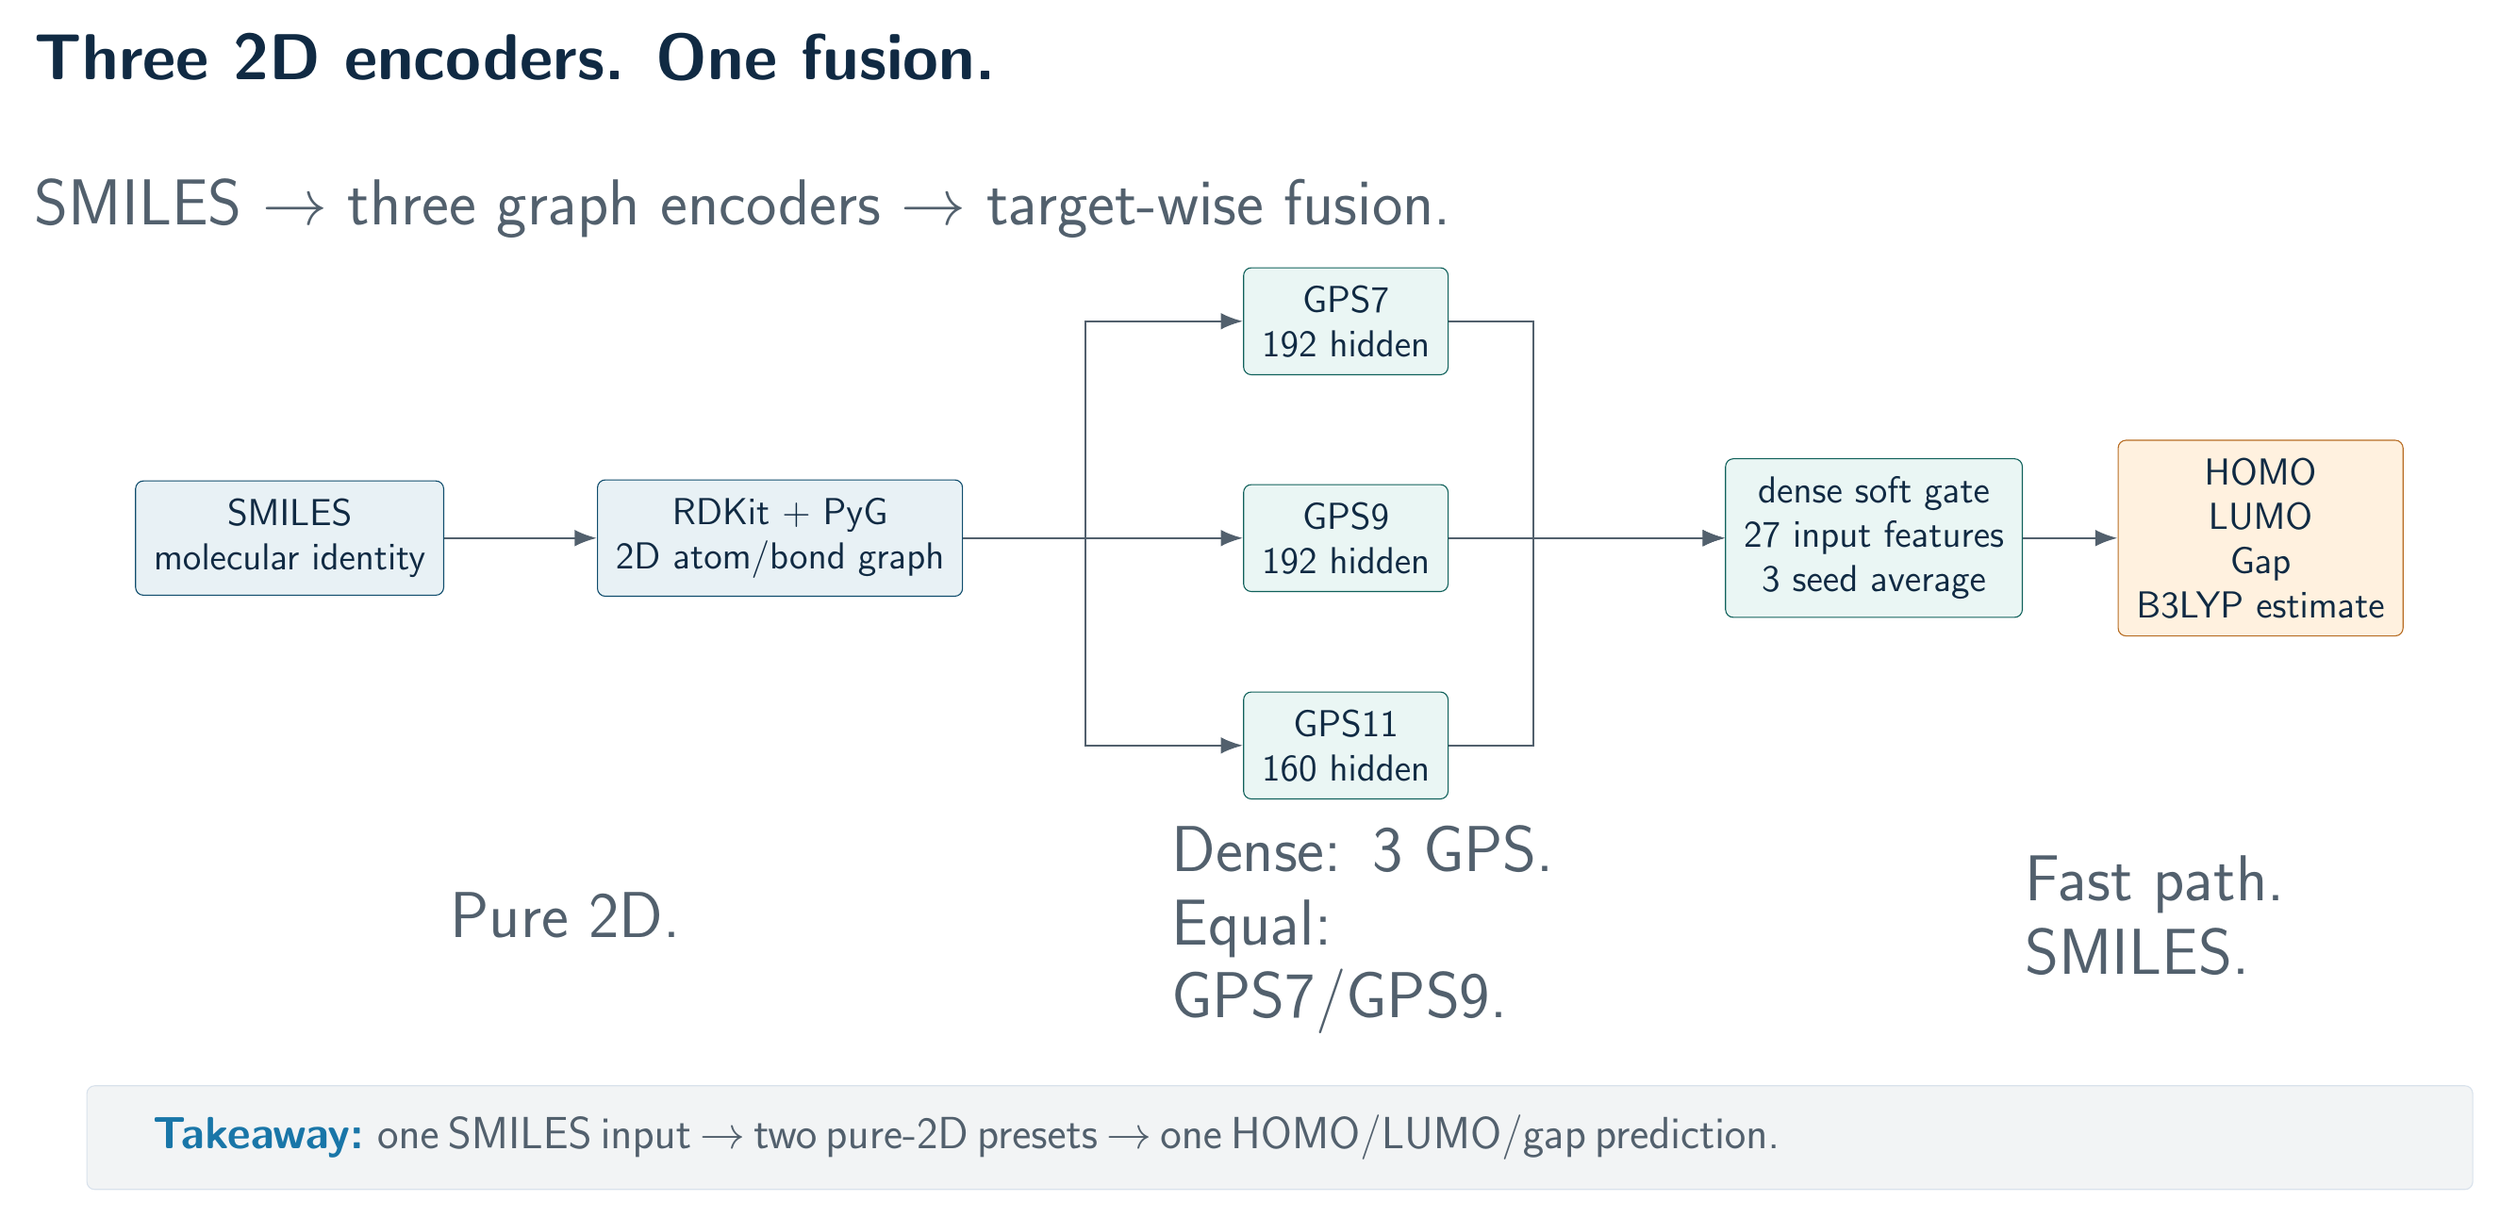
\begin{tikzpicture}[x=1in,y=1in]
  \node[title,font=\sffamily\bfseries\fontsize{108}{120}\selectfont,anchor=west] at (0,6.25) {Three 2D encoders. One fusion.};
  \node[subtitle,font=\sffamily\fontsize{38}{45}\selectfont,anchor=west] at (0,5.45) {SMILES $\rightarrow$ three graph encoders $\rightarrow$ target-wise fusion.};

  \node[box,font=\sffamily\fontsize{14}{17}\selectfont,minimum width=2.4cm,minimum height=1.0cm] (smiles) at (1.4,3.70) {SMILES\\molecular identity};
  \node[box,font=\sffamily\fontsize{14}{17}\selectfont,minimum width=2.4cm,minimum height=1.0cm] (rdkit) at (4.0,3.70) {RDKit + PyG\\2D atom/bond graph};
  \node[model,font=\sffamily\fontsize{14}{17}\selectfont,minimum width=2.25cm,minimum height=1.0cm] (g7) at (7.0,4.85) {GPS7\\192 hidden};
  \node[model,font=\sffamily\fontsize{14}{17}\selectfont,minimum width=2.25cm,minimum height=1.0cm] (g9) at (7.0,3.70) {GPS9\\192 hidden};
  \node[model,font=\sffamily\fontsize{14}{17}\selectfont,minimum width=2.25cm,minimum height=1.0cm] (g11) at (7.0,2.60) {GPS11\\160 hidden};
  \node[model,font=\sffamily\fontsize{14}{17}\selectfont,minimum width=2.7cm,minimum height=1.15cm] (gate) at (9.8,3.70) {dense soft gate\\27 input features\\3 seed average};
  \node[specialist,font=\sffamily\fontsize{14}{17}\selectfont,minimum width=2.55cm,minimum height=1.15cm] (out) at (11.85,3.70) {HOMO\\LUMO\\Gap\\B3LYP estimate};

  \draw[arrow] (smiles.east) -- (rdkit.west);
  \draw[arrow] (rdkit.east) -- ++(0.65,0) |- (g7.west);
  \draw[arrow] (rdkit.east) -- ++(0.65,0) -- (g9.west);
  \draw[arrow] (rdkit.east) -- ++(0.65,0) |- (g11.west);
  \draw[arrow] (g7.east) -- ++(0.45,0) |- (gate.west);
  \draw[arrow] (g9.east) -- (gate.west);
  \draw[arrow] (g11.east) -- ++(0.45,0) |- (gate.west);
  \draw[arrow] (gate.east) -- (out.west);

  \node[note,font=\sffamily\fontsize{23}{28}\selectfont,text width=3.8cm] at (3.0,1.70) {Pure 2D.};
  \node[note,font=\sffamily\fontsize{23}{28}\selectfont,text width=5.2cm] at (7.1,1.62) {Dense: 3 GPS.\\Equal:\\GPS7/GPS9.};
  \node[note,font=\sffamily\fontsize{23}{28}\selectfont,text width=3.8cm] at (11.35,1.70) {Fast path.\\SMILES.};
  \node[draw=grid, fill=futureFill, text=muted, rounded corners=3pt, minimum width=12.65in, minimum height=.55in, align=left, inner sep=7pt, text width=11.95in] at (6.65,0.52) {\sffamily\fontsize{16}{19}\selectfont\textcolor{blue}{\bfseries Takeaway:} one SMILES input $\rightarrow$ two pure-2D presets $\rightarrow$ one HOMO/LUMO/gap prediction.};
\end{tikzpicture}
\end{document}
